%\section{Problem 3.13}
\mysection{3.13}{Problem 3.13}

\numberwithin{equation}{subsection}

A Gaussian product channel $Y_j = g_j X_j + Z_j$, $j\in \{1,2\}$ with $g_1 < g_2$ and average power constraint $P$ is given. We want to know above what power $P^*$ we start to use both channels and what are the features of the \textit{energy-per-bit-rate function} $E_b(R)$.

\subsection{Optimal power allocation}

We notice that to achieve the maximum capacity from the channel we have to solve the following optimization problem
%
\begin{equation}\label{optproblem}
\begin{aligned}
&\max_{P_j} && \sum_{j=1}^2 \frac{1}{2} \cdot \log(1+g_j^2 \cdot P_j)\\
&\text{subject to}&& -P_j \leq 0 \quad j\in \{1,2\} \\
& 		   && \sum_{j=1}^2 P_j - P = 0
\end{aligned}
\end{equation}

%In order to solve \eqref{optproblem} we build the following equation
%%
%\begin{equation}
%	\nabla_{P_j}\Big\{-\sum_{j=1}^2 \frac{1}{2} \cdot \log(1+g_j^2 \cdot P_j) + \sum_{j=1}^2 \lambda_j \cdot (-P_j) + \nu \cdot \Big(\sum_{j=1}^2 P_j - P\Big)  \Big\} = 0
%	\label{f0}
%\end{equation}
%
%Solving \eqref{f0} we obtain what follows.
%
%\begin{equation}
%	\begin{gathered}
%		\frac{1}{2} \cdot \frac{1}{P_j+\frac{1}{g_j^2}}+\lambda_j-\nu=0 \\
%		\Rightarrow \frac{1}{2} \cdot \frac{1}{P_j+\frac{1}{g_j^2}} \leq \nu = \frac{1}{2\mu}
%	\end{gathered}
%\end{equation}
%
%\begin{equation}
%	\begin{gathered}
%		\sum_{j=1}^2 \max\Big\{\mu - \frac{1}{g_j^2},0\Big\} = P \\
%		\Rightarrow \mu = \frac{P}{2}+\frac{1}{2g_1^2} + \frac{1}{2g_2^2}
%	\end{gathered}
%\end{equation}
%
%\begin{equation}
%	\begin{gathered}
%	 P_j = \max\Big\{\mu - \frac{1}{g_j^2},0\Big\} \\
%	 \Rightarrow P_1= \max\Big\{\frac{P}{2} + \frac{1}{2g_2^2} - \frac{1}{2g_1^2},0\Big\} = \begin{cases}
%	  \frac{P}{2} + \frac{1}{2g_2^2} - \frac{1}{2g_1^2} \quad P \geq \frac{1}{g_1^2} - \frac{1}{g_2^2} \\
%		0 \quad P < \frac{1}{g_1^2} - \frac{1}{g_2^2}
%	 \end{cases} \\
%	 \Rightarrow P_2= \max\Big\{\frac{P}{2} + \frac{1}{2g_1^2} - \frac{1}{2g_2^2},0\Big\} = \frac{P}{2} + \frac{1}{2g_1^2} - \frac{1}{2g_2^2} \quad \forall \quad P \geq 0
%	\end{gathered}
%\end{equation}
%
%We conclude that the second channel is opened for every amount of allocated power $P$ while the first channel is opened only if and only if \eqref{Pcondition} is verified.
%
%\begin{equation}
%	P \geq \frac{1}{g_1^2} - \frac{1}{g_2^2}
%	\label{Pcondition}
%\end{equation}

The solution of this problem is the classical water filling solution, i.e.
%
\begin{equation} \label{eq:3.13_Popt}
P_j^{opt} = \qty[ \mu - \frac{1}{g_j^2}]^+ = \max \qty{ \mu - \frac{1}{g_j^2},0}
\end{equation}
%
where $\mu$ is obtained from
%
\begin{equation} \label{eq:3.13_mu}
\sum_{j=1}^d \qty[\mu - \frac{1}{g_j^2}]^+ = P
\end{equation}
%
and the capacity obtained is
%
\begin{equation} \label{eq:3.13_capacity}
C = \sum_{j=1}^d C(g_j^2P_j) = \frac{1}{2}\sum_{j=1}^d [\log(g_j^2P_j)]^+
\end{equation}

Now, since we want both channels to be used (in particular the the first channel since it's the worst one), we need to impose the cutoff $\mu > \frac{1}{g_j^2}$. Thus, from Eq.~\eqref{eq:3.13_mu} we obtain $2\mu-\frac{1}{g_1^2}-\frac{1}{g_2^2}=P$ $\Rightarrow \, \mu = \frac{1}{2}\qty( P+\frac{1}{g_1^2}+\frac{1}{g_2^2} )$, which, united with the inequality on $\mu$, yields
%
\begin{equation}
P > \frac{1}{g_1^2}-\frac{1}{g_2^2}
\end{equation}
%
obtaining a channel capacity equal to
%
\begin{align}
\begin{split}
C =& \sum_{j=1}^2 C(g_j^2P_j) = \frac{1}{2}[\log(g_1^2\mu) + \log(g_2^2\mu)]\\
=& \frac{1}{2}\log\qty( g_1^2 g_2^2 \frac{1}{4}\qty( P+\frac{1}{g_1^2}+\frac{1}{g_2^2} )^2 )
\end{split}
\end{align}

\subsection{Energy-per-bit-rate function computation}

Now we want to compute the \textit{energy-per-bit-rate function} $E_b(R)$ in the scenario previously described. We know that $P = R \cdot E$ where $R$ is the \textit{bit-rate} of the channel and $E$ is the used energy for every bit. In addition we know that the \textit{bit-rate} is bounded by the channel capacity
%
\begin{equation} \label{eq:rate_bound}
R \leq
	\begin{cases}
	\frac{1}{2} \log\big( 1 + g_2^2P \big) & P \leq \frac{1}{g_1^2} - \frac{1}{g_2^2}\\
	\frac{1}{2}\log\qty( \frac{g_1^2 g_2^2}{4}\qty( P+\frac{1}{g_1^2}+\frac{1}{g_2^2} )^2 ) & P > \frac{1}{g_1^2} - \frac{1}{g_2^2}
	\end{cases}
\end{equation}

Let's consider the first case, which is the case where only channel 2 is opened. Writing $P$ in function of $R$ we get what follows and considering the bound with equality we get
%
\begin{equation}
P \geq \Big(\frac{2^{2R}-1}{g_2^2}\Big)
\end{equation}
%
which only holds for low transmitting power, i.e. $P\leq \frac{1}{g_1^2} - \frac{1}{g_2^2}$ which in terms of bitrate means $R \leq \log_2 \qty(\frac{g_2}{g_1})$ (obtained substituting the power bound on Eq.~\eqref{eq:rate_bound}).

Similarly we obtain
%
\begin{equation}
	\begin{gathered}
		P \geq \Big(\frac{2^{R+1}}{g_1g_2} -\frac{1}{g_1^2} - \frac{1}{g_2^2} \Big)
		\quad \text{if} \quad R >  \log\Big(\frac{g_2}{g_1}\Big)
	\end{gathered}
\end{equation}

Knowing that $P = E \cdot R$ we define the \textit{energy-per-bit-rate function} $E_b(R)$ as shown in \eqref{epbfunction}.

\begin{equation} E_b(R)=
	\begin{cases}
		\frac{1}{R}\Big(\frac{2^{2R}-1}{g_2^2}\Big) & R \leq \log\Big(\frac{g_2}{g_1}\Big) \\
		\frac{1}{R} \Big(\frac{2^{R+1}}{g_1g_2} -\frac{1}{g_1^2} - \frac{1}{g_2^2} \Big) & R > log\Big(\frac{g_2}{g_1}\Big)
	\end{cases}
	\label{epbfunction}
\end{equation}

Now we want to show that the function \eqref{epbfunction} is strictly monotonically increasing and convex on $R$. To do so we first compute the first and the second derivatives of the function itself.

\begin{equation}
	E'_b(R)= \begin{cases}
		\frac{1}{R^2g_2^2} \Big(2^{2R}(2R\ln(2)-1)+1\Big) & R \leq \log\Big(\frac{g_2}{g_1}\Big) \\
		\frac{1}{R^2g_1^2 g_2^2} \Big(2^{R+1} g_1 g_2 ( R \ln(2)-1)+g_1^2+g_2^2 \Big) & R > log\Big(\frac{g_2}{g_1}\Big)
\end{cases}
\end{equation}
%
\begin{equation}
	E''_b(R)= \begin{cases}
		\frac{1}{R^3g_2^2} \Big(2^{2R}(4R^2\ln(2)^2 -2R \ln(2)+1)-1\Big)  & R \leq \log\Big(\frac{g_2}{g_1}\Big) \\
		\frac{1}{R^3 g_1 g_2} \Big( 2^{R+1} g_1 g_2 ( R^2 \ln(2)^2 - R \ln(2) +1 ) -g_1^2 -g_2^2 \Big) & R > log\Big(\frac{g_2}{g_1}\Big)

\end{cases}
\end{equation}

\begin{figure}[t]
	\centering
	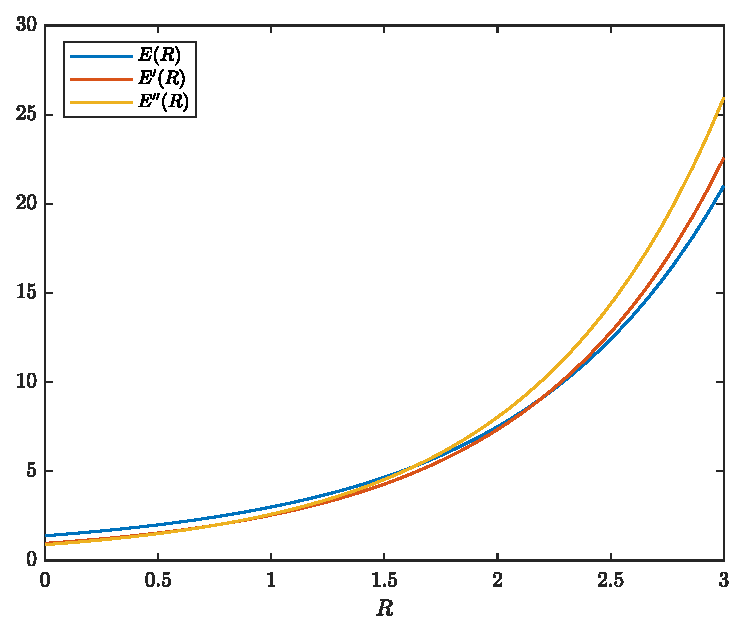
\includegraphics[width=0.7\linewidth]{img/energy_per_bit_1.eps}
	\caption{$E_b(R)$, $E'_b(R)$, $E''_b(R)$ for $R \leq \log\Big(\frac{g_2}{g_1}\Big)$ }
	\label{fig:funcex2}
\end{figure}

Note that these derivatives are pretty difficult to manage analytically. Fortunately, for low rates both derivatives are only a function of $R$ and multiplied by a constant positive factor $1/g_2^2$ which doesn't change the sign. Thus, we can see from Fig.~\ref{fig:funcex2} that at least for $R \leq \log\Big(\frac{g_2}{g_1}\Big)$, $E_b(R)$ is strictly increasing and convex. It can also be shown that the function is continuous on the splitting condition but showing anything analytically or even graphically on the second part of the function is not really easy since there is also the dependence from both $g_1$ and $g_2$. The only clear thing is that for $R \rightarrow \infty$ both derivatives are positive.

Now we want to compute the minimum energy-per-bit as $R \rightarrow 0$. We notice that for low values of $R$ we find ourself in the case where only one of the two channels is opened. Then to compute $\lim_{R \rightarrow 0} E_b(R)$ we proceed as follows.
%
\begin{equation}
	\lim_{R \rightarrow 0} E_b(R) =
		\lim_{R \rightarrow 0} \Big(\frac{2^{2R}-1}{g_2^2 R}\Big) = \lim_{R \rightarrow 0} \frac{ \frac{d(2^{2R}-1)}{dR}} {\frac{dg_2^2 R}{dR}}=\frac{2\ln{2}}{g_2^2}
		\label{emin}
\end{equation}

\numberwithin{equation}{section}
